\newpage
%Unknown4: -Pollution ... can it be avoided
%Leo: Very immature !!!: Text unfinished; structure weak.
%leo: Context seems to describe the solution
%Leo: Solution is composed of 2 solutions
%Leo: Unclear use of "systems" ==> see p.8.
%Leo: Some requirement on logging (Why described here?)(Why these?)
%Leo: Fig. 5 seems to describe solution 2 only 
\section*{CENTRALIZED SYSTEM LOGGING}

%Roland: Generally this was seen as the weakest pattern
%Peter: why do system administrators want logging?

%Unknown3: Centralized <-- To what purpose?
%Unknown3: System <-- Distributed?
%Unknown3: Why it needed? 

The application needs to provide the ability of logging certain events or actions 
%Leo: seems to be the solution to sub 1:
by using the built in system logging of a platform. 

\begin{center}
\ding{118} \ding{118} \ding{118}
\end{center}

\textbf{Having a variety of logging formats and log-file locations makes it hard to monitor the state of a whole enterprise, including all running applications.}\\

\textit{Format Variety.} A high variety of logging formats increases the complexity of integrating the information held within those several log files. It becomes a burden to nullify
%Peter: nullify?? --> analyse
the different lay-outs of these log files.\\ 

%Peter: reconsider
\textit{Location Variety.} When having a variety of log file locations the dispersion of those locations makes it hard to find those log files.
%difficult to gather those files into one location.\\

\textit{Information Granularity.} Not only the formats might be varying, but also the granularity of information. This makes it hard to monitor all applications in a consistent way or to integrate the information in a consistent way for other statistical purposes like e.g. root cause analysis \cite{conf/mkwi/PaschkeS06}.

\begin{center}
\ding{118} \ding{118} \ding{118} 
\end{center}

%Rebecca: Don't agree with this (Roland, navragen bij Rebecca)
\textbf{Therefore:
%Leo: sub 1
Use the built-in system logging mechanism whenever possible.
%Leo: sub 2
If it is not possible, then define a standard format to be used by all systems 
%Leo: what do you mean with 'systems'? --> Systems, OR: Subsystems of one application, OR: platform systems
and implement your own logger.}\\
%Peter: ..., ..., OS-defined logger

Many monitoring tools use the system built-in logging mechanisms. The connection between these is well defined and proven. It is therefore of help for the system administrators if these built-in logging mechanisms are used by all applications, as this allows the administrators to make use of existing tools (e.g. Nagios\footnote{\url{http://www.nagios.org/}} or HP OpenView\footnote{\url{http://www.openview.hp.com/}}) that collect, centralize, and search the logs \cite{Limoncelli2011a}.

The built-in system logging mechanisms take care of the log file location problem. They also prescribe the format, thereby forcing the developers, but also supporting them, to make consistent use of logging on the appropriate granularity.

It is also a lot easier to automatically generate incidents from specific defined events from the built-in system log for an IT service management (ITSM) tool. This ITSM tool can be configured to forward the automatically generated incidents directly, without human intervention, to the second line specialists. This way incidents are more easily solved without less human intervention, saving valuable time of the system administrators.

Of course logging in many cases has to be activated from within the system, so developers often have to explicitly program it into the system. But using the built-in logging mechanism alone does not ensure that the developers also make use of logging when it is appropriate. To address this issue guidelines could be defined and used by the developers for including logging in the system. 

%Leo: unfinished sentences
%Leo: Structure unclear

If it is not possible to use the built-in system logging, e.g. because of different operating systems being used, then develop your own {\sc Diagnostic Logger} \cite{Harrison2011} and define a standard for your system landscape that works good in combination with the administration tools being used. Use the properties of built-in system logging mechanisms as basis for the requirements of your own logging mechanism. The most important point hereby is that this mechanism can be connected to the ITSM tools used by the system administrators. Ensure that this standard system is used for logging. This approach can be combined with {\sc Single File Location}.
%Rebecca: Consequences? Should logging mean 1 log or logging in a centralized location? Use of logging services. What about log files.

%Leo: Some? 3 REQ's <-- ?
Some requirements a good log should met to be valuable are\footnote{\url{http://gojko.net/2006/12/09/logging-anti-patterns/}}:
\begin{itemize}
	\item Log actions before they happen.
	\item Mind the file size if logs should be copied or archived.
	\item Split messages into different files depending on intended audience/way of using.
\end{itemize}

%Unknown1: the relationships between the studied patterns and the related patterns are not clear. We use the term 'uplent'(?). What about Dependency and Composition?? Abstraction (pattern language).
On the type of usage it depends how robust the chosen solution acts within daily use:
\begin{itemize}
	\item When normal availability is desirable one can choose, when the  centralized logging system fails, to recover the server and reload the logging of the several subsystems
	\item When high availability is needed the centralized logging system needs to be made so, e.g. as a High Availability cluster
\end{itemize}
Otherwise the chosen solution could become a Single Point of Failure (SPoF).

For implementing a (system) logging facility one can make use of {\sc  Factory} \cite{Gamma95}, which makes it possible to create loggers ({\sc  Adapters} \cite{Gamma95}) for different applications. See figure \ref{fig:systemLogging}. Becasue one wants just one instance of a system logger, {\sc  Singleton} \cite{Gamma95} is the preferent way to implement it.
%Peter: bad for testing logging! Parameterize.

\begin{figure}[h]
\centering
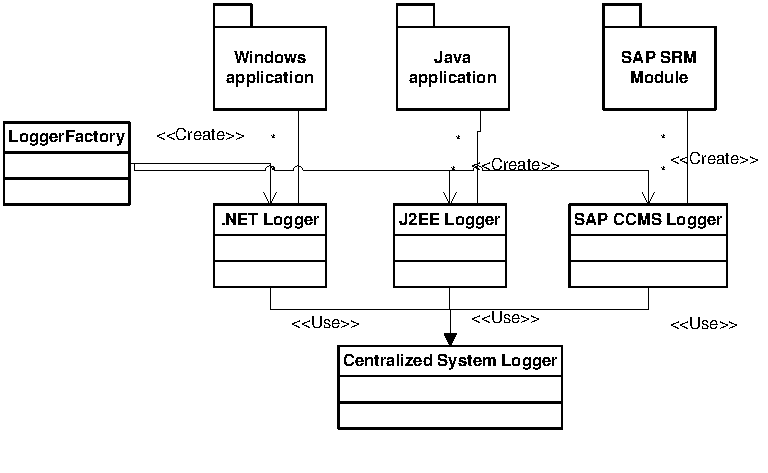
\includegraphics{patterns/systemLoggingDiagram.pdf}
\caption{Main solution structure of CENTRALIZED SYSTEM LOGGING}
\label{fig:systemLogging}
\end{figure}
%Leo: Pattern, Sub 2?
%Leo: <<Use>>?
%Leo: --> Centralized System Logger <-- Open arrow? - subtype?

%Toelichting: An event possibly created by a monitoring tool or the application itself takes the role of anOriginator CareTaker needs to be logged (saved within aMemento) ...

\begin{center}
\ding{118} \ding{118} \ding{118} 
\end{center}

%Rebecca: All patterns should be in a consistent form. This is different than others. (Roland)
Known Uses:\\
Many monitoring tools provide a mechanism for gathering several logs to one central place, but even easier to use is a distributed log collector:
\begin{itemize}
	\item Scribe\footnote{\url{https://github.com/facebook/Scribe}} is a scalable log aggregation server used and released by Facebook as open source. Scribe is written in C++ and uses Thrift\footnote{\url{http://thrift.apache.org/}} for the protocol encoding. Since it uses thrift, virtually any language can work with it.
	\item Flume\footnote{\url{https://cwiki.apache.org/FLUME/}} is an Apache project for collecting, aggregating, and moving large amounts of log data. It stores all this data on HDFS\footnote{\url{http://hadoop.apache.org/docs/stable/hdfs_design.html}}.
\end{itemize}

As an example of the implementation of {\sc Centralized System Logging} we have performed with our second year students System and Network Engineering some practical scripting exercises with Python where they, amongst others, use some standard libraries available for Python to log events to the system event log and afterwards create a statistical plot of it with the help of the Python library Matplotlib.\footnote{\url{http://matplotlib.org/}} 
An example of a call from Python to the Windows system log is:

%\begin{minted}[mathescape,
%               linenos,
%               numbersep=5pt,
%               gobble=2,
%               frame=lines,
%               framesep=2mm]{python}
               
\lstset{language=Python}

%Peter: J Avgs top article bad API
\begin{lstlisting}

import win32evtlogutil
win32evtlogutil.ReportEvent(ApplicationName, EventID, EventCategory,
    		EventType, Inserts, Data, SID)

\end{lstlisting}

%\end{minted}

This way the students get a feeling for how to integrate information from several resources (systems and applications) into one central store (system event log) and transform that information into a graphical output which could give insighs into e.g. the number of incidents per month with error level ERROR.




